% Options for packages loaded elsewhere
\PassOptionsToPackage{unicode}{hyperref}
\PassOptionsToPackage{hyphens}{url}
%
\documentclass[
]{article}
\usepackage{amsmath,amssymb}
\usepackage{lmodern}
\usepackage{iftex}
\ifPDFTeX
  \usepackage[T1]{fontenc}
  \usepackage[utf8]{inputenc}
  \usepackage{textcomp} % provide euro and other symbols
\else % if luatex or xetex
  \usepackage{unicode-math}
  \defaultfontfeatures{Scale=MatchLowercase}
  \defaultfontfeatures[\rmfamily]{Ligatures=TeX,Scale=1}
\fi
% Use upquote if available, for straight quotes in verbatim environments
\IfFileExists{upquote.sty}{\usepackage{upquote}}{}
\IfFileExists{microtype.sty}{% use microtype if available
  \usepackage[]{microtype}
  \UseMicrotypeSet[protrusion]{basicmath} % disable protrusion for tt fonts
}{}
\makeatletter
\@ifundefined{KOMAClassName}{% if non-KOMA class
  \IfFileExists{parskip.sty}{%
    \usepackage{parskip}
  }{% else
    \setlength{\parindent}{0pt}
    \setlength{\parskip}{6pt plus 2pt minus 1pt}}
}{% if KOMA class
  \KOMAoptions{parskip=half}}
\makeatother
\usepackage{xcolor}
\IfFileExists{xurl.sty}{\usepackage{xurl}}{} % add URL line breaks if available
\IfFileExists{bookmark.sty}{\usepackage{bookmark}}{\usepackage{hyperref}}
\hypersetup{
  pdftitle={final report},
  pdfauthor={Rui Miao},
  hidelinks,
  pdfcreator={LaTeX via pandoc}}
\urlstyle{same} % disable monospaced font for URLs
\usepackage[margin=1in]{geometry}
\usepackage{color}
\usepackage{fancyvrb}
\newcommand{\VerbBar}{|}
\newcommand{\VERB}{\Verb[commandchars=\\\{\}]}
\DefineVerbatimEnvironment{Highlighting}{Verbatim}{commandchars=\\\{\}}
% Add ',fontsize=\small' for more characters per line
\usepackage{framed}
\definecolor{shadecolor}{RGB}{248,248,248}
\newenvironment{Shaded}{\begin{snugshade}}{\end{snugshade}}
\newcommand{\AlertTok}[1]{\textcolor[rgb]{0.94,0.16,0.16}{#1}}
\newcommand{\AnnotationTok}[1]{\textcolor[rgb]{0.56,0.35,0.01}{\textbf{\textit{#1}}}}
\newcommand{\AttributeTok}[1]{\textcolor[rgb]{0.77,0.63,0.00}{#1}}
\newcommand{\BaseNTok}[1]{\textcolor[rgb]{0.00,0.00,0.81}{#1}}
\newcommand{\BuiltInTok}[1]{#1}
\newcommand{\CharTok}[1]{\textcolor[rgb]{0.31,0.60,0.02}{#1}}
\newcommand{\CommentTok}[1]{\textcolor[rgb]{0.56,0.35,0.01}{\textit{#1}}}
\newcommand{\CommentVarTok}[1]{\textcolor[rgb]{0.56,0.35,0.01}{\textbf{\textit{#1}}}}
\newcommand{\ConstantTok}[1]{\textcolor[rgb]{0.00,0.00,0.00}{#1}}
\newcommand{\ControlFlowTok}[1]{\textcolor[rgb]{0.13,0.29,0.53}{\textbf{#1}}}
\newcommand{\DataTypeTok}[1]{\textcolor[rgb]{0.13,0.29,0.53}{#1}}
\newcommand{\DecValTok}[1]{\textcolor[rgb]{0.00,0.00,0.81}{#1}}
\newcommand{\DocumentationTok}[1]{\textcolor[rgb]{0.56,0.35,0.01}{\textbf{\textit{#1}}}}
\newcommand{\ErrorTok}[1]{\textcolor[rgb]{0.64,0.00,0.00}{\textbf{#1}}}
\newcommand{\ExtensionTok}[1]{#1}
\newcommand{\FloatTok}[1]{\textcolor[rgb]{0.00,0.00,0.81}{#1}}
\newcommand{\FunctionTok}[1]{\textcolor[rgb]{0.00,0.00,0.00}{#1}}
\newcommand{\ImportTok}[1]{#1}
\newcommand{\InformationTok}[1]{\textcolor[rgb]{0.56,0.35,0.01}{\textbf{\textit{#1}}}}
\newcommand{\KeywordTok}[1]{\textcolor[rgb]{0.13,0.29,0.53}{\textbf{#1}}}
\newcommand{\NormalTok}[1]{#1}
\newcommand{\OperatorTok}[1]{\textcolor[rgb]{0.81,0.36,0.00}{\textbf{#1}}}
\newcommand{\OtherTok}[1]{\textcolor[rgb]{0.56,0.35,0.01}{#1}}
\newcommand{\PreprocessorTok}[1]{\textcolor[rgb]{0.56,0.35,0.01}{\textit{#1}}}
\newcommand{\RegionMarkerTok}[1]{#1}
\newcommand{\SpecialCharTok}[1]{\textcolor[rgb]{0.00,0.00,0.00}{#1}}
\newcommand{\SpecialStringTok}[1]{\textcolor[rgb]{0.31,0.60,0.02}{#1}}
\newcommand{\StringTok}[1]{\textcolor[rgb]{0.31,0.60,0.02}{#1}}
\newcommand{\VariableTok}[1]{\textcolor[rgb]{0.00,0.00,0.00}{#1}}
\newcommand{\VerbatimStringTok}[1]{\textcolor[rgb]{0.31,0.60,0.02}{#1}}
\newcommand{\WarningTok}[1]{\textcolor[rgb]{0.56,0.35,0.01}{\textbf{\textit{#1}}}}
\usepackage{longtable,booktabs,array}
\usepackage{calc} % for calculating minipage widths
% Correct order of tables after \paragraph or \subparagraph
\usepackage{etoolbox}
\makeatletter
\patchcmd\longtable{\par}{\if@noskipsec\mbox{}\fi\par}{}{}
\makeatother
% Allow footnotes in longtable head/foot
\IfFileExists{footnotehyper.sty}{\usepackage{footnotehyper}}{\usepackage{footnote}}
\makesavenoteenv{longtable}
\usepackage{graphicx}
\makeatletter
\def\maxwidth{\ifdim\Gin@nat@width>\linewidth\linewidth\else\Gin@nat@width\fi}
\def\maxheight{\ifdim\Gin@nat@height>\textheight\textheight\else\Gin@nat@height\fi}
\makeatother
% Scale images if necessary, so that they will not overflow the page
% margins by default, and it is still possible to overwrite the defaults
% using explicit options in \includegraphics[width, height, ...]{}
\setkeys{Gin}{width=\maxwidth,height=\maxheight,keepaspectratio}
% Set default figure placement to htbp
\makeatletter
\def\fps@figure{htbp}
\makeatother
\setlength{\emergencystretch}{3em} % prevent overfull lines
\providecommand{\tightlist}{%
  \setlength{\itemsep}{0pt}\setlength{\parskip}{0pt}}
\setcounter{secnumdepth}{-\maxdimen} % remove section numbering
\ifLuaTeX
  \usepackage{selnolig}  % disable illegal ligatures
\fi

\title{final report}
\author{Rui Miao}
\date{2022-04-22}

\begin{document}
\maketitle

\hypertarget{a.-introduction}{%
\section{A. Introduction}\label{a.-introduction}}

There are many different factors that affects the salary level of
employers working in a company, such as degree, experience, number of
years working in the company, gender, and so on. In this research, we
are interested in the factors affecting the salary level of Data
Scientists. According to a journal Research administrator salary:
association with education, experience, credentials, and gender{[}1{]},
we expect a positive relationship between experience and salary level,
and male tends to have a higher salary than female.

\hypertarget{a.-purpose-of-the-research}{%
\subsection{a. Purpose of the
Research:}\label{a.-purpose-of-the-research}}

The purpose of the research comes from the fact that as statistics
students, we are curious about careers related and their prospects. This
will provide us with some insights into my future career path and what
to expect.

The importance of the research is that most third-year students are
preparing to find an internship in the near future. And salary level is
one of the most essential factors that we will consider to select a job.
Thus, we are interested in studying the factors which may affect the
salary level.

\hypertarget{b.-research-question}{%
\subsection{b. Research Question:}\label{b.-research-question}}

\textbf{How does salary relate to years of experience, years at the
company, and gender?}

We are interested in this specific research question since answering
this question can give us a preliminary understanding of our possible
future development working in a company. Besides, we are also interested
in whether there is gender discrimination when it comes to the salaries
of male data scientists and female data scientists.

Our goal for this research is to build a statistical model which is best
for explaining the relationship between salary, and other possible
predictors. And we may use our model to predict the salary that we may
receive in out future career.

\hypertarget{c.-background-of-the-dataset}{%
\subsection{c.~Background of the
Dataset}\label{c.-background-of-the-dataset}}

This dataset{[}2{]} is found on the website \emph{Kaggle} containing
salary records from top companies. There are in total 62642 observations
and 29 variables in our original dataset. We are interested in the
question \emph{How does salary relate to years of experience, years at
the company, and gender?}. Thus, the variables that we are interested in
are \emph{salary}, \emph{yearatcompany}, \emph{yearsofexperience} and
\emph{gender}.

\newpage

\hypertarget{b.-methods}{%
\section{B. Methods}\label{b.-methods}}

\hypertarget{a.-how-and-when-the-data-was-acquired}{%
\subsection{a. How and When the data was
acquired}\label{a.-how-and-when-the-data-was-acquired}}

The data was scraped off levels.fyi and then cleaned by the author. The
license{[}3{]} of this data set is including in the \emph{Reference}
section. According to the terms and conditions of the website, people
may use the data for personal, non-commercial purposes (mentioned in the
last sentence in the ``License'' section).

\hypertarget{b.-cleaning-and-wrangling-the-data}{%
\subsection{b. Cleaning and Wrangling the
Data}\label{b.-cleaning-and-wrangling-the-data}}

There are in total 62642 observations and 29 variables in our original
dataset. After filtering out unrelated titles and leaving only
observations with Data Scientist as title, observations with missing
values in gender and ``Other'' in gender are also filtered out. As one
of the purposes of our analysis is to explore whether there is gender
discrimination in salaries. The size of the dataset shrinks to 1718
observations. We are only interested in exploring 12 of the 29 variables
including \emph{salary}, \emph{yearatcompany}, \emph{yearsofexperience}
\emph{gender, Bachelors\_Degree, Masters\_Degree, Doctorate\_Degree,
Some\_College, Highschool, Race\_Asian, Race\_White,} and
\emph{Race\_Black}. We mutated the gender to a numeric values, where
male is 0, and female is 1 so that we could interpret the gender data
more easily.

\begin{itemize}
\item
  \textbf{title}: A categorical variable representing the job title of
  an individual in his/her company. Since we are interested in the
  titles related to our future careers, ``title'' can give us
  information about specific titles that we are interested in.
\item
  \textbf{totalyearlycompensation(*1000)}: A numerical variable
  representing the total annual compensation of an individual with title
  in his/her company. According to our research question, this is our
  response variable. It will be denoted as salary in the following
  analysis for simplicity.
\item
  \textbf{yearatcompany}: A numerical variable representing the number
  of years that an individual has worked in his/her company. According
  to our research question, this is one of our predictors.
\item
  \textbf{yearsofexperience}: A numerical variable representing the
  number of years of an individual's working experience. According to
  our research question, this is one of our predictors. gender: A
  categorical variable representing the gender of an individual.
  According to our research question, this is one of our predictors.
\item
  \textbf{gender:} A categorical variable representing the gender of
  individual
\item
  \textbf{Bachelors\_Degree}: A categorical variable representing if an
  individual has a bachelor's degree.
\item
  \textbf{Masters\_Degree}: A categorical variable representing if an
  individual has a master's degree.
\item
  \textbf{Doctorate\_Degree}: A categorical variable representing if an
  individual has a doctor's degree.
\item
  \textbf{Some\_College}: A categorical variable representing if an
  individual has a college's degree.
\item
  \textbf{Highschool}: A categorical variable representing if an
  individual has a high school's degree.
\item
  \textbf{Race\_Asian}: A categorical variable representing if the race
  of an individual is Asian.
\item
  \textbf{Race\_Black}: A categorical variable representing if the race
  of an individual is black.
\item
  \textbf{Race\_White}: A categorical variable representing if the race
  of an individual is white.

  \newpage
\end{itemize}

\begin{Shaded}
\begin{Highlighting}[]
\NormalTok{knitr}\SpecialCharTok{::}\FunctionTok{kable}\NormalTok{(}\FunctionTok{describe}\NormalTok{(datascience), }\AttributeTok{align =} \StringTok{\textquotesingle{}l\textquotesingle{}}\NormalTok{, }\AttributeTok{caption =} \StringTok{"SUmmary Table for the variables"}\NormalTok{)}
\end{Highlighting}
\end{Shaded}

\begin{longtable}[]{@{}
  >{\raggedright\arraybackslash}p{(\columnwidth - 26\tabcolsep) * \real{0.1791}}
  >{\raggedright\arraybackslash}p{(\columnwidth - 26\tabcolsep) * \real{0.0373}}
  >{\raggedright\arraybackslash}p{(\columnwidth - 26\tabcolsep) * \real{0.0373}}
  >{\raggedright\arraybackslash}p{(\columnwidth - 26\tabcolsep) * \real{0.0896}}
  >{\raggedright\arraybackslash}p{(\columnwidth - 26\tabcolsep) * \real{0.0896}}
  >{\raggedright\arraybackslash}p{(\columnwidth - 26\tabcolsep) * \real{0.0522}}
  >{\raggedright\arraybackslash}p{(\columnwidth - 26\tabcolsep) * \real{0.0896}}
  >{\raggedright\arraybackslash}p{(\columnwidth - 26\tabcolsep) * \real{0.0672}}
  >{\raggedright\arraybackslash}p{(\columnwidth - 26\tabcolsep) * \real{0.0299}}
  >{\raggedright\arraybackslash}p{(\columnwidth - 26\tabcolsep) * \real{0.0299}}
  >{\raggedright\arraybackslash}p{(\columnwidth - 26\tabcolsep) * \real{0.0448}}
  >{\raggedright\arraybackslash}p{(\columnwidth - 26\tabcolsep) * \real{0.0821}}
  >{\raggedright\arraybackslash}p{(\columnwidth - 26\tabcolsep) * \real{0.0970}}
  >{\raggedright\arraybackslash}p{(\columnwidth - 26\tabcolsep) * \real{0.0746}}@{}}
\caption{SUmmary Table for the variables}\tabularnewline
\toprule
\begin{minipage}[b]{\linewidth}\raggedright
\end{minipage} & \begin{minipage}[b]{\linewidth}\raggedright
vars
\end{minipage} & \begin{minipage}[b]{\linewidth}\raggedright
n
\end{minipage} & \begin{minipage}[b]{\linewidth}\raggedright
mean
\end{minipage} & \begin{minipage}[b]{\linewidth}\raggedright
sd
\end{minipage} & \begin{minipage}[b]{\linewidth}\raggedright
median
\end{minipage} & \begin{minipage}[b]{\linewidth}\raggedright
trimmed
\end{minipage} & \begin{minipage}[b]{\linewidth}\raggedright
mad
\end{minipage} & \begin{minipage}[b]{\linewidth}\raggedright
min
\end{minipage} & \begin{minipage}[b]{\linewidth}\raggedright
max
\end{minipage} & \begin{minipage}[b]{\linewidth}\raggedright
range
\end{minipage} & \begin{minipage}[b]{\linewidth}\raggedright
skew
\end{minipage} & \begin{minipage}[b]{\linewidth}\raggedright
kurtosis
\end{minipage} & \begin{minipage}[b]{\linewidth}\raggedright
se
\end{minipage} \\
\midrule
\endfirsthead
\toprule
\begin{minipage}[b]{\linewidth}\raggedright
\end{minipage} & \begin{minipage}[b]{\linewidth}\raggedright
vars
\end{minipage} & \begin{minipage}[b]{\linewidth}\raggedright
n
\end{minipage} & \begin{minipage}[b]{\linewidth}\raggedright
mean
\end{minipage} & \begin{minipage}[b]{\linewidth}\raggedright
sd
\end{minipage} & \begin{minipage}[b]{\linewidth}\raggedright
median
\end{minipage} & \begin{minipage}[b]{\linewidth}\raggedright
trimmed
\end{minipage} & \begin{minipage}[b]{\linewidth}\raggedright
mad
\end{minipage} & \begin{minipage}[b]{\linewidth}\raggedright
min
\end{minipage} & \begin{minipage}[b]{\linewidth}\raggedright
max
\end{minipage} & \begin{minipage}[b]{\linewidth}\raggedright
range
\end{minipage} & \begin{minipage}[b]{\linewidth}\raggedright
skew
\end{minipage} & \begin{minipage}[b]{\linewidth}\raggedright
kurtosis
\end{minipage} & \begin{minipage}[b]{\linewidth}\raggedright
se
\end{minipage} \\
\midrule
\endhead
totalyearlycompensation & 1 & 1718 & 199.5768335 & 106.4453764 & 182.50
& 187.9738372 & 77.83650 & 10 & 900 & 890 & 1.5735207 & 4.4431619 &
2.5681195 \\
yearsofexperience & 2 & 1718 & 4.9039581 & 4.0889323 & 4.00 & 4.3655523
& 2.96520 & 0 & 30 & 30 & 1.5845878 & 3.6337717 & 0.0986503 \\
yearsatcompany & 3 & 1718 & 1.9875437 & 2.2138323 & 1.75 & 1.6159884 &
1.85325 & 0 & 19 & 19 & 2.3463805 & 8.5670322 & 0.0534113 \\
gender* & 4 & 1718 & 1.2101281 & 0.4075180 & 1.00 & 1.1380814 & 0.00000
& 1 & 2 & 1 & 1.4217935 & 0.0215102 & 0.0098318 \\
Bachelors\_Degree & 5 & 1718 & 0.1344587 & 0.3412438 & 0.00 & 0.0436047
& 0.00000 & 0 & 1 & 1 & 2.1411588 & 2.5860671 & 0.0082329 \\
Masters\_Degree & 6 & 1718 & 0.4150175 & 0.4928685 & 0.00 & 0.3938953 &
0.00000 & 0 & 1 & 1 & 0.3446480 & -1.8823124 & 0.0118910 \\
Doctorate\_Degree & 7 & 1718 & 0.1868452 & 0.3899007 & 0.00 & 0.1090116
& 0.00000 & 0 & 1 & 1 & 1.6053963 & 0.5776345 & 0.0094068 \\
Some\_College & 8 & 1718 & 0.0005821 & 0.0241262 & 0.00 & 0.0000000 &
0.00000 & 0 & 1 & 1 & 41.3764131 & 1711.0034914 & 0.0005821 \\
Highschool & 9 & 1718 & 0.0017462 & 0.0417634 & 0.00 & 0.0000000 &
0.00000 & 0 & 1 & 1 & 23.8468914 & 567.0042689 & 0.0010076 \\
Race\_Asian & 10 & 1718 & 0.2904540 & 0.4541041 & 0.00 & 0.2383721 &
0.00000 & 0 & 1 & 1 & 0.9223613 & -1.1499179 & 0.0109558 \\
Race\_White & 11 & 1718 & 0.1827707 & 0.3865909 & 0.00 & 0.1039244 &
0.00000 & 0 & 1 & 1 & 1.6402076 & 0.6906841 & 0.0093270 \\
Race\_Black & 12 & 1718 & 0.0075669 & 0.0866836 & 0.00 & 0.0000000 &
0.00000 & 0 & 1 & 1 & 11.3550015 & 127.0099881 & 0.0020913 \\
\bottomrule
\end{longtable}

As shown, total yearly compensation ranges from 10000 to 900000 which is
a large interval. And we noticed that the median is slightly lower than
the mean, implying that the distribution of salary might be left-skewed.
And the table illustrates that the variance of salary is much larger
than the variances of our predictors, which coincides with our
large-interval finding of salary in Table 1.

Also the mean of year of experience is longer than the mean of year at
company, which may indicates that employees usually have worked in
different companies. And according to the values of \emph{skew}, we
noticed that all of the three numeric variables are right-skewed in
different level.

Based on the mean of Bachelor's degree,there are about 13\% of the
population (excluding the na) that have obtained a bachelor's degrees,
while there are about 42\% of the population (excluding the na) that
have obtained a master's degree, and there are about 19\% of the
population (excluding the na) have obtained a doctor's degree. Also,
Asian are the most popular race in this dataset.

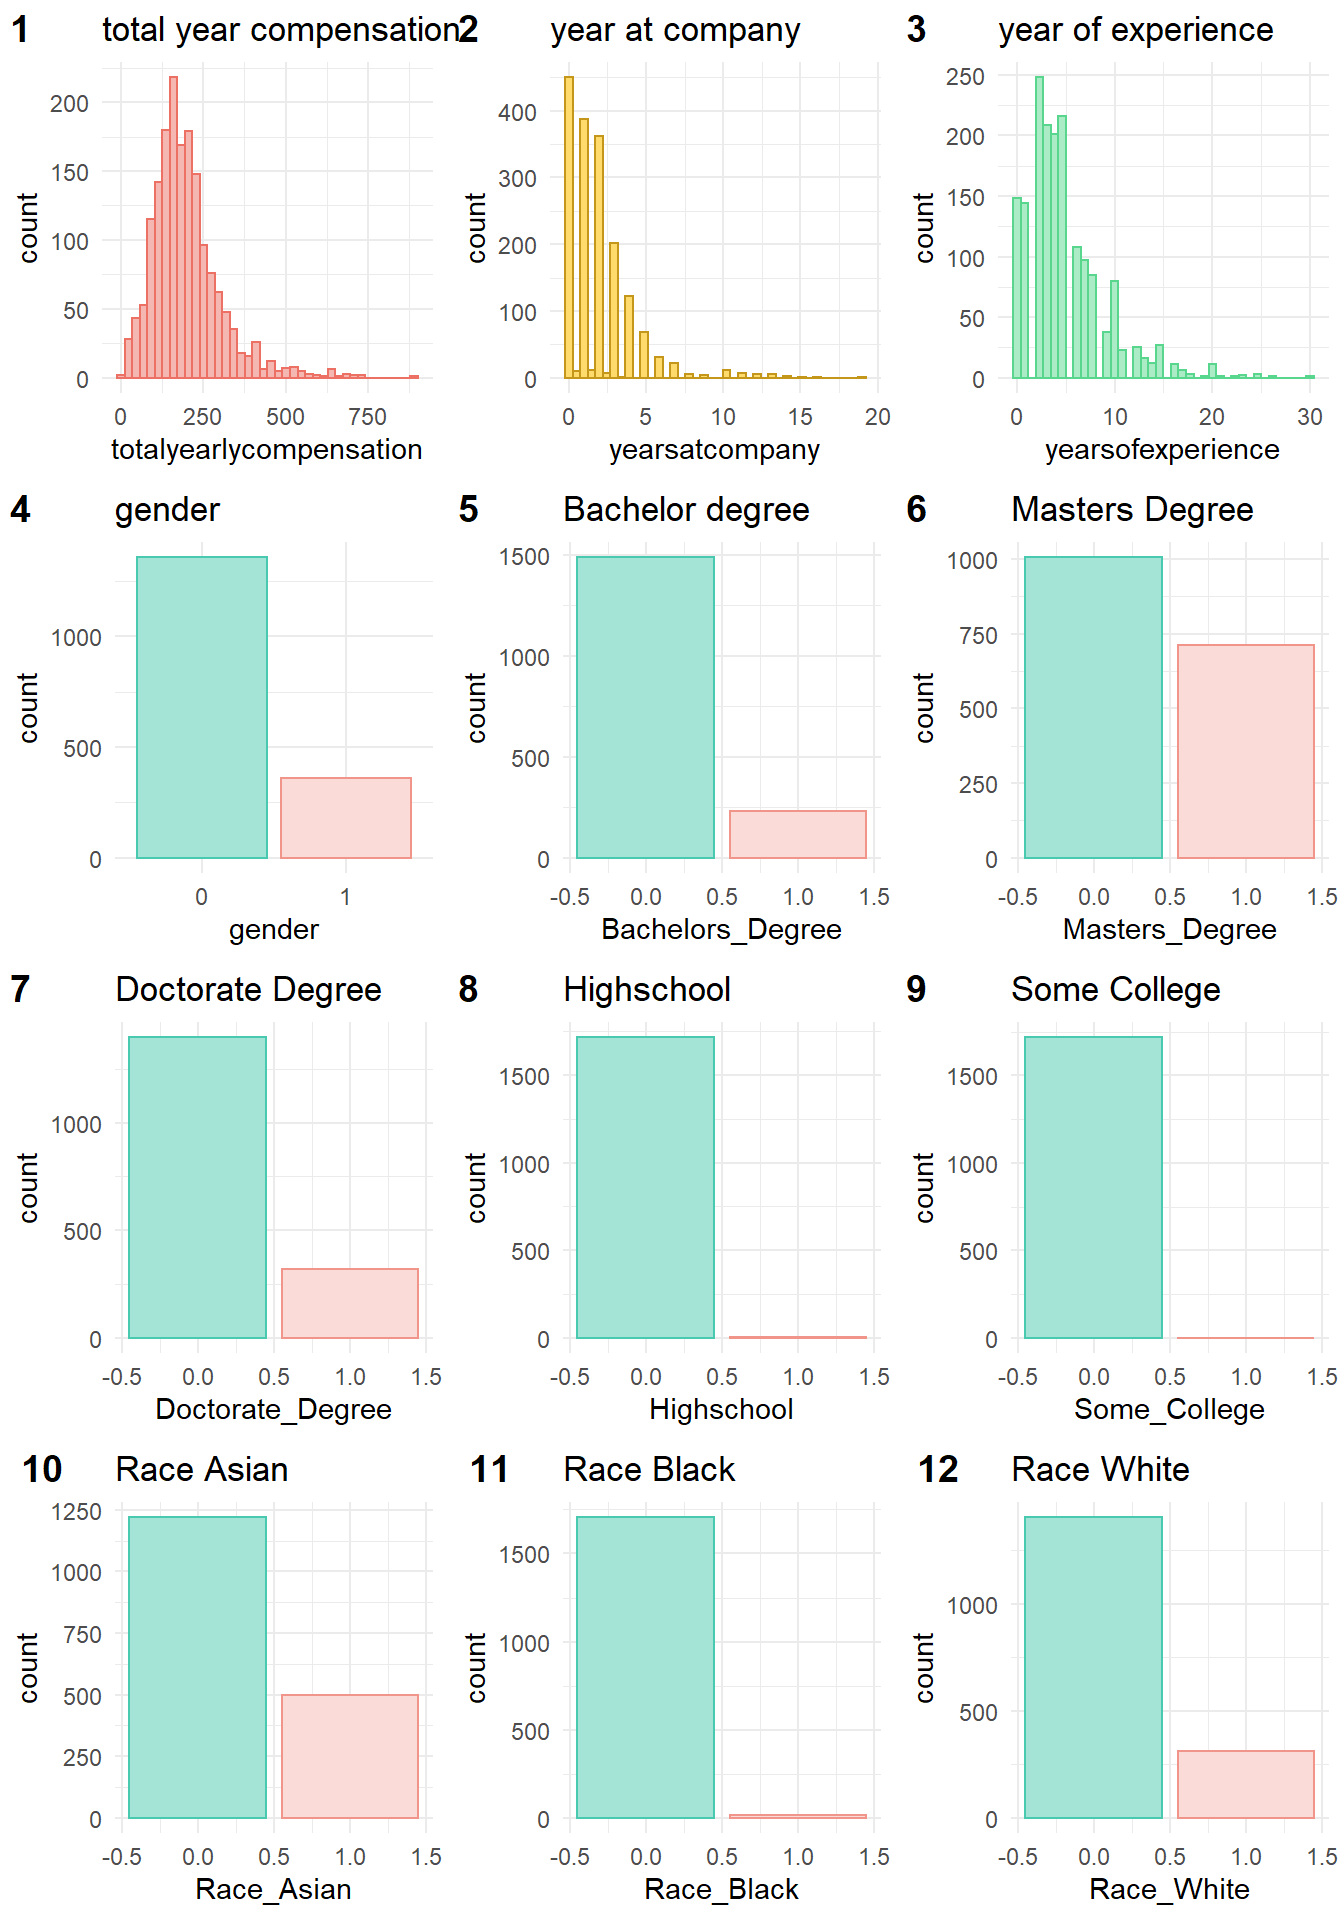
\includegraphics{final-report_files/figure-latex/unnamed-chunk-1-1.pdf}

Figure 1 showing the distribution of salary indicates a left-skewed
trend with some outliers on the right, which have salaries over
5\emph{105dollars per year. Most values concentrate in the interval
between 10000 and 4}105. There are 35 observations that have a salary
above 5*105. Since they are likely to affect the result of our linear
model, we may remove them when fitting a linear model.

Figure 2 (years of experience) and Figure 3 (years at company) display a
similar trend as Figure 1 (salary). They are even more left-skewed than
salary and have a few outliers as well, for instance, the 41 people with
more than 15 years of experience and the 44 people with more than 7
years at the same company.

Figure 4 (gender) illustrates a strong gender imbalance. There are fewer
than 400 female data scientists and more than 1200 male data scientists
in our dataset.

From the figures shown, we can see that our continuous predictors
including years of experience and years at the company have similar
distribution as our response variable, which justifies the use of linear
regression in the analysis.

\hypertarget{c.-variable-selection}{%
\subsection{c.~Variable Selection:}\label{c.-variable-selection}}

\hfill\break
To build a model, the first thing to start with is selecting reasonable
predictors and responses that could provide an answer to the research
question. Firstly, a linear model with all possible and reasonable
variables related to the research question was fitted. Based on this
model, we calculated the p-values for each predictors, and removed the
predictors randomly until all the predictors have been checked.\\
ANOVA partial F-Test and T-Test were used to evaluate if those
predictors can be removed.

\begin{itemize}
\item
  if the p-value of ANOVA partial F-Test is\\

  \begin{itemize}
  \tightlist
  \item
    \textless{} 0.05, use T − T est to make further decision\\
  \item
    \textgreater{} 0.05, the predictors should be removed
  \end{itemize}
\item
  if the p-value of T-Test is\\
  -- \textless{} 0.05, the predictors cannot be removed\\
  -- \textgreater{} 0.05, the predictors should be removed

  All the predictors that cannot be removed are the appropriate
  variables to build our model.
\end{itemize}

\hypertarget{d.-analyze-the-data}{%
\subsection{d.~Analyze the data}\label{d.-analyze-the-data}}

My research question can be answered using a \textbf{linear regression}
model because we expect that there exists a linear relationship between
our predictors and responses. And each row of our data represents an
independent individual, which indicates that each row in our dataset
should be independent to one another.

I will be using \textbf{total yearly compensation (Y)} as my response
and use the predictors \textbf{years of experience (}\(X_1\)\textbf{)},
\textbf{years at the company (}\(X_2\)\textbf{)}, \textbf{gender
(}\(X_3\)\textbf{),} \textbf{Bachelors\_Degree}(\(X_4\)),
\textbf{Masters\_Degree}(\(X_5\)), \textbf{Doctorate\_Degree}(\(X_6\))
because we are interested in the annual salary level which is total
yearly compensation, and we would like to see how years of experience,
years at company and gender affect the total yearly compensation.

Some anticipated issues might be that the outliers have some impact when
estimating the coefficients of our model and need to be removed. Another
issue is that two of our predictor variables, years of experience and
years at the company might be correlated to each other in a way that
years of experience = years at the company + years at other companies.
In fact, there are 543 individuals whose years of experience are exactly
equal to their years at the company. The correlation between our
predictor variables will make our prediction less accurate.

\newpage

\hypertarget{c.-result}{%
\section{C. Result}\label{c.-result}}

\hypertarget{process-of-obtaining-the-final-model}{%
\subsubsection{1. Process of obtaining the final
model}\label{process-of-obtaining-the-final-model}}

After removing the variables with insignificant p-values (except Genders
since we are interested in gender), the \textbf{ANOVA} partial
\textbf{F-Test} is in-significant. Thus, all these predictors can be
removed. For the remaining variables, w checked one by one, and for
removing every one of them, the values of AN OV A partial F-Test is
significant, which indicate that all the remaining cannot be removed.
Then the model is only having predictors \emph{yearatcompany},
\emph{yearofexperience}, \emph{gender, Bachelors degree, Masters degree,
and Doctorate degree, and response totalyearlycompensation}.

\hypertarget{goodness-of-the-result}{%
\subsubsection{2. Goodness of the result}\label{goodness-of-the-result}}

\begin{center}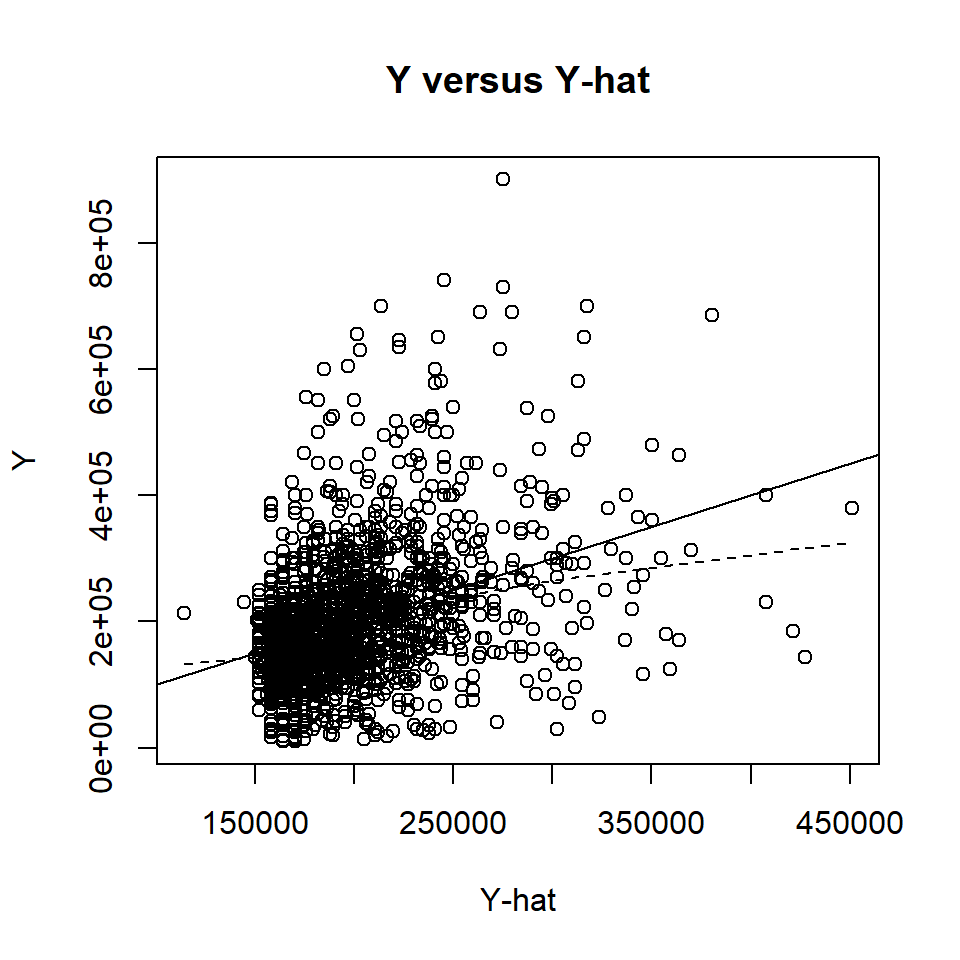
\includegraphics{final-report_files/figure-latex/Response versus fitted values-1} \end{center}

The plot above showing the relationship between the response Y and the
fitted values of Y. By observing the plot of response against the fitted
values, we see that there is a non-random scatter around the identity
function, indicating that there is not a simple function of a linear
combination of predictors. And most of the points in the graph are
having a positive values. Thus, conditional means response is not a
perfect single function of a linear combination of the predictors.

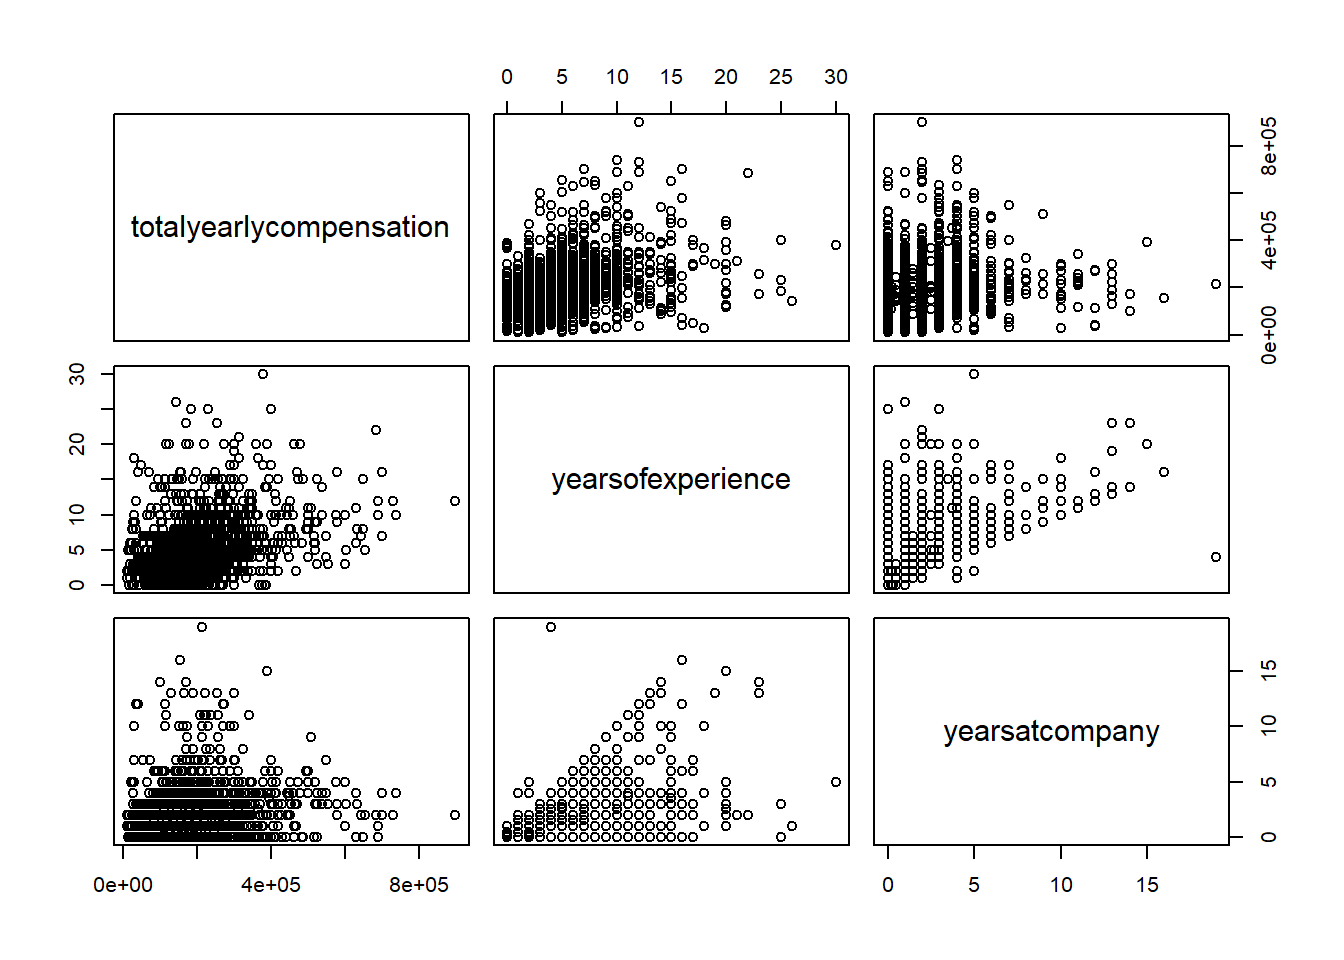
\includegraphics{final-report_files/figure-latex/unnamed-chunk-2-1.pdf}

Based on this plot, we noticed that there is some patterns between each
pairs of variables. Most of the plots have points concentrating at the
lower left and moving upward to the upper-right corner. Therefore, most
of the associations between each possible pairs of the association is
positive. Only the scatter plot for total yearly compensation and years
at company seems to have an unclear association. Above this, we can
conclude that conditional mean of each predictor has a linear function
with another predictor.

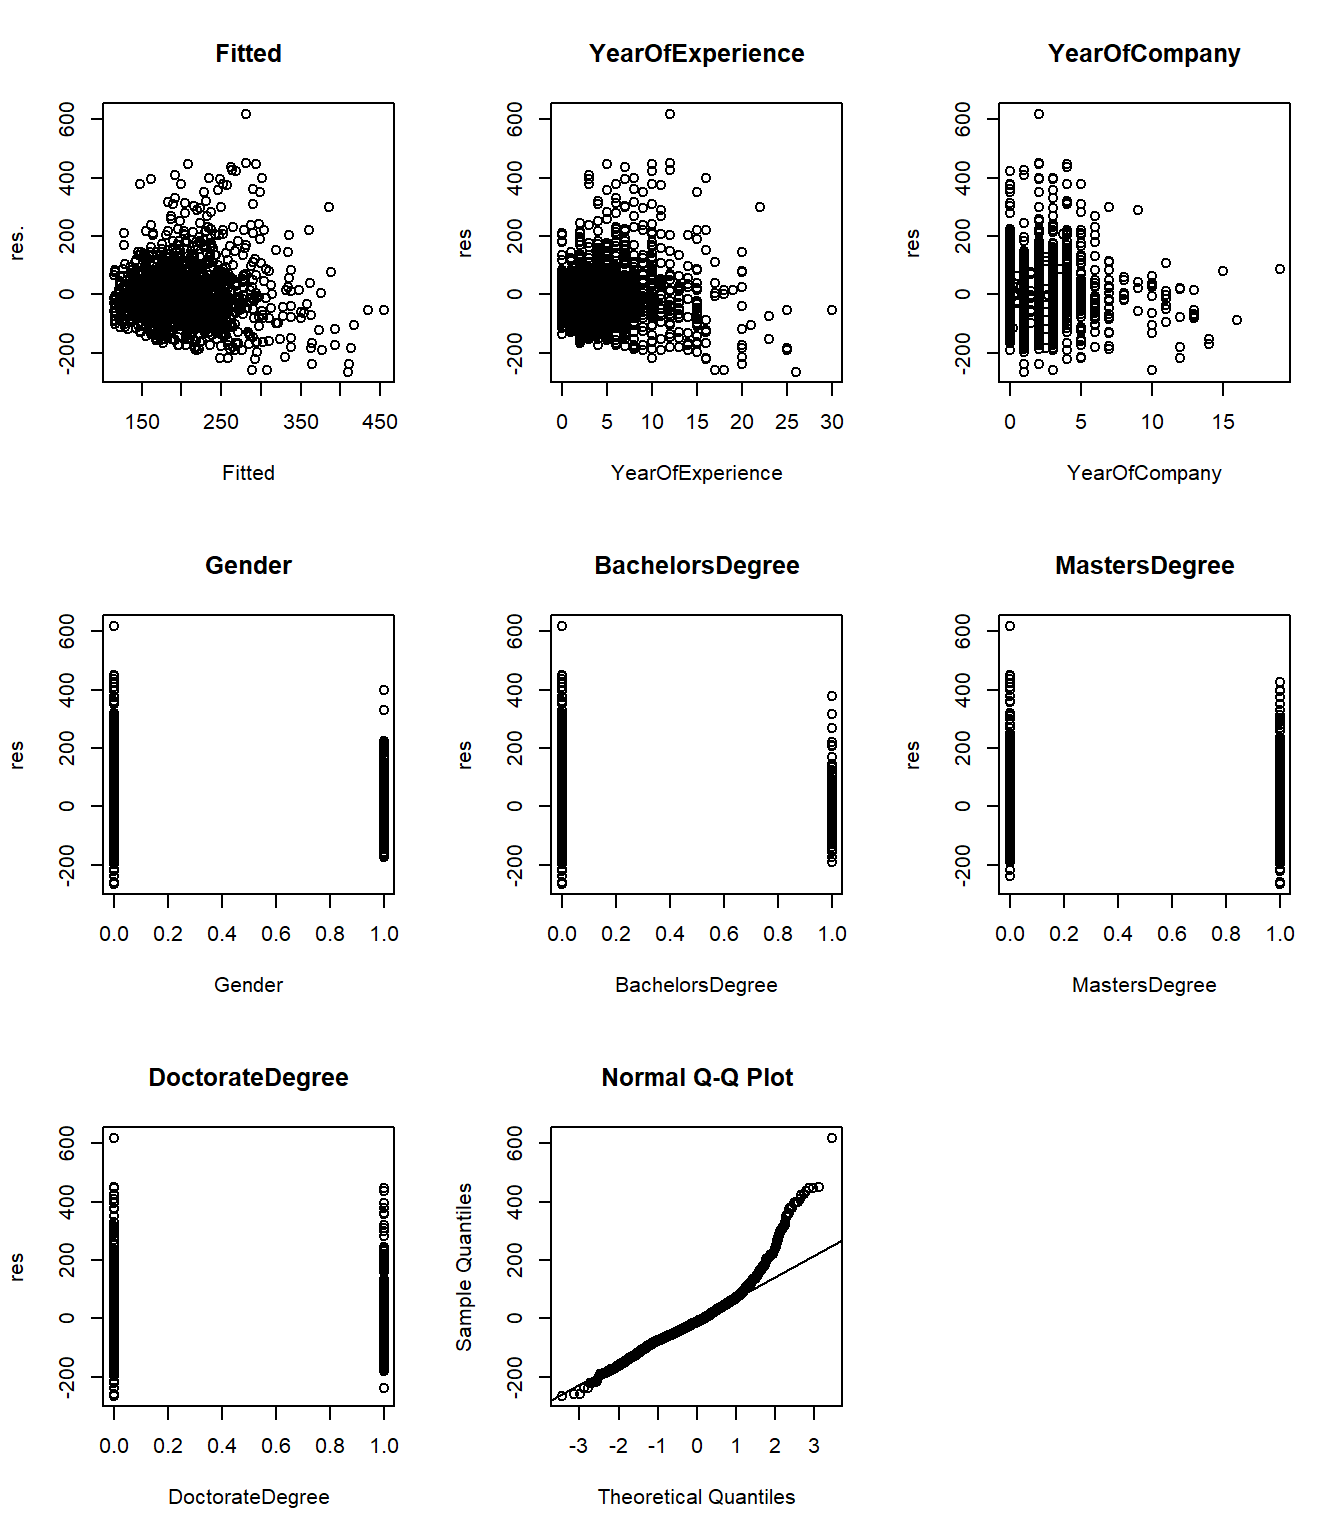
\includegraphics{final-report_files/figure-latex/unnamed-chunk-3-1.pdf}

We recognized that the scatters does not spread randomly and equally.
But we noticed that all the points are more equally distributed at both
side of 0,. This implies that \textbf{assumptions 1} is likely
satisfied, which is the population errors have mean zero. However,
assumption 2, 3 still do not hold perfectly, which are the population
responses (equivalently errors) are somhow correlated with each other,
and the population errors (equivalently responses) do not have constant
spread/variance around conditional mean.

By the normal QQ-plot, there is a straight diagonal string of points
along an identity function, with some deviation on both ends. This shows
that there is a \textbf{normality}, the populations errors are normally
distributed with the mean of assumption 1.

\begin{verbatim}
##                            term   Estimate Std. Error    t value      Pr(>|t|)
## 1                   (Intercept) 165.033014  5.2529025 31.4174908 1.923442e-171
## 2 datascience$yearsofexperience  10.415917  0.6497583 16.0304484  5.460427e-54
## 3    datascience$yearsatcompany  -4.183001  1.1953335 -3.4994428  4.781718e-04
## 4  datascience$Bachelors_Degree -48.450760  7.6040814 -6.3716783  2.397603e-10
## 5    datascience$Masters_Degree -22.281666  5.5454344 -4.0180200  6.123390e-05
## 6  datascience$Doctorate_Degree  41.485401  6.7276924  6.1663642  8.699036e-10
## 7           datascience$gender1  -1.003891  5.6693093 -0.1770746  8.594707e-01
\end{verbatim}

This is the summary table of our model. Based on the p-values in the
table, we noticed that the p-values for \textbf{year of experience} and
\textbf{year at company} are extremely small, which indicates that these
two are two main factors of the salary level.

\hypertarget{d.-conclusion-and-summary}{%
\section{D. Conclusion and Summary}\label{d.-conclusion-and-summary}}

The most significant factors that would affect salary are years working
at company, years of experience, Gender.

The relationships between response and each predictors are as follow:

\begin{itemize}
\item
  years working at company: negative
\item
  years of experience: positive
\item
  genders: positive
\end{itemize}

According to the above relationships, we are not surprising to see that
if you are more experienced, you will earn more.

However, there are some interesting facts that for people works longer
in a company, they will earn less. This could be caused by some
extremely outliers in the dataset. Usually, employees will at least stay
at the same salary level through out the duration of working at the
companies. Another one is that people having a bachelor's or master's
degree earn less than those does not have. All the information of degree
are recorded by 0 and 1 without NA. Thus, 0 may be the default values
for the column, which may represents not having that degree or unknown.
This may influence the result and cause the interesting facts.

Another funny fact is that female earns more than males. Because from
many facts of gender inequality in reality, females earn less than males
at the same positions, with same degree. I think this may show an
improvement in the gender equality nowadays. Another reason may be the
percentage of female in this dataset is much smaller than male, thus,
the data of female in this dataset is less representative. However, I
would like to believe that we have a more open, less descrimination
working environment for female than in the past.

Overall, only according to the result, experience is the most important
factors to earn more. And generally, females earns more than males when
working as a datascientists.

\newpage

\hypertarget{f.-reference}{%
\section{F. Reference}\label{f.-reference}}

{[}1{]} Shambrook, Jennifer, et al.~\emph{``Research administrator
salary: association with education, experience, credentials, and
gender.''} Journal of Research Administration, vol.~42, no. 2, fall
2011, pp.~87+. Gale In Context: Canada,

\href{https://go.gale.com/ps/i.dop=CICu=utorontomainid=GALEA276807849v=2.1it=rsid=bookmark-CICasid=809af152}{\emph{https://go.gale.com/ps/i.dop=CICu=utorontomainid=GALEA276807849v=2.1it=rsid=bookmark-CICasid=809af152}}\emph{.}

{[}2{]} ``Data Science and STEM Salaries'', Kaggle.com, 2021.
{[}Online{]}.

Available:
\href{https://www.kaggle.com/jackogozaly/data-science-and-stem-salaries}{\emph{https://www.kaggle.com/jackogozaly/data-science-and-stem-salaries}}\emph{.}

{[}3{]} License: According to the terms and conditions of the website,
people may use the data for personal, non-commercial purposes (mentioned
in the last sentence in the ``License'' section). This is the link to
the page of terms and conditions of level.fyi:

\href{https://www.levels.fyi/about/terms.html}{\emph{https://www.levels.fyi/about/terms.html}}

\end{document}
